\documentclass{hebutthesis}

\begin{document}

\pdfbookmark[section]{论文标题}{cover}  %在生成的PDF文档中创建书签
% !TeX root = ../HebutThesis_example.tex(此文件是被HebutThesis_example.tex调用的)
\title{论文标题}
\author{作者姓名}
\studentID{000000}
\college{学院}
\major{专业}
\supervisor{指导老师姓名 \qquad 指导老师职称}
\hebutThesisTime{2xxx年x月x日}
\maketitle
      %插入封面
\pdfbookmark[section]{摘要}{abstract}
% !TeX root = ../HebutThesis_example.tex(此文件是被HebutThesis_example.tex调用的)
% 在此文件中编辑摘要页里需要填写的内容

\pagenumbering{Roman}   % 页面用罗马字体编号

% 中文摘要和关键词
\newpage
\begin{center}
    \fontsize{18}{1}\fzxbsjt{毕业设计(论文)中文摘要}
\end{center}
\begin{tcolorbox}
\begin{center}
    {\fontsize{16}{0}\heiti{\textbf{您的论文题目}}}   % 此处修替换为您的论文题目
\end{center}
\vspace{8mm}
% 中文摘要
\noindent
{\fontsize{16}{0}\heiti{\textbf{摘要:}}}
\vspace{2mm}
\setlength{\parindent}{24pt}
  % 此处替换为您的中文摘要内容,另起一段需要空一行

  本科毕业设计论文摘要是对整个研究工作的高度概括,
  通常包含研究的背景、目的、方法、主要结果和结论。
  具体写法应简洁明了,遵循以下步骤:

  1、背景:简短介绍研究领域和研究的意义。

  2、目的:明确指出研究旨在解决的问题或目标。

  3、方法:概述采用的研究方法或技术。

  4、结果:简要描述研究的主要发现或成果。

  5、结论:提出研究的主要结论,可能包括对未来研究的建议。

  本科毕业设计论文的关键词应精准概括论文的核心内容和研究领域,
  有助于读者和数据库检索系统快速理解和定位论文。写法要点如下:

  1、相关性:选择与论文主题紧密相关的词汇。

  2、专业性:使用专业领域内常用的术语或词汇。

  3、具体性:避免过于宽泛的词汇,关键词应具体反映论文的研究内容。

  4、数量:一般选取3-5个关键词,足以覆盖论文的主要研究领域和特点。

  5、排序:按照关键词的重要程度或与论文内容的相关性排序。

  关键词之间用逗号分隔,放在摘要下方,
  有时候也可以包括研究方法和地点等信息,
  以提高论文的可检索性。
  
\vspace{8mm}

% 中文关键词
\noindent
{\fontsize{12}{0}\heiti\textbf{关键词}}: \quad 关键词 1 \quad 关键词 2 \quad 关键词 3  % 此处替换为您的中文关键词
\end{tcolorbox}

% 外文摘要和关键词
\newpage
\begin{center}
    \fontsize{18}{1}\songti{毕业设计(论文)外文摘要}
\end{center}
\begin{tcolorbox}
\pdfbookmark[section]{ABSTRACT}{ABSTRACT}
\begin{center}
    \fontsize{14}{0}\songti{\textbf{Your Thesis Title}}   % 此处替换为您的论文外文标题
\end{center}
\vspace{8mm}
% 外文摘要
\noindent
{\fontsize{16}{0}\heiti{\textbf{ABSTRACT}}}
\vspace{2mm}
\setlength{\parindent}{24pt}
  % 此处替换为您的外文摘要内容,另起一段需要空一行

  The abstract of the undergraduate graduation thesis is a high-level summary of the entire research work, usually including the background of the research
  Purpose, Method, Main Results, and Conclusion. The specific writing should be concise and clear, following the following steps:
  1. Background: Briefly introduce the research field and its significance.
  2. Purpose: Clearly indicate the problem or goal that the research aims to solve.
  3. Method: Summarize the research methods or techniques used.
  4. Result: Briefly describe the main findings or outcomes of the study.
  5. Conclusion: Present the main conclusions of the study, which may include recommendations for future research.

  The keywords for undergraduate graduation thesis should accurately summarize the core content and research field of the thesis, which is helpful for reading
  Quickly understand and locate papers through the database retrieval system. The key points of writing are as follows:
  1. Relevance: Choose vocabulary closely related to the topic of the paper.
  2. Professionalism: Using commonly used terms or vocabulary in the professional field.
  3. Specific: Avoid overly broad vocabulary, and keywords should specifically reflect the research content of the paper.
  Separate keywords with commas and place them below the abstract, sometimes including research methods and locations
  Information to improve the searchability of the paper.

\vspace{8mm}

% 外文关键词
\noindent
{\fontsize{12}{0}\heiti\textbf{Keywords}}: keyword 1, keyword 2, keyword 3    % 此处替换为您的外文关键词
% \vspace{28mm}
\end{tcolorbox}

\setlength{\parindent}{24pt}

   %插入摘要
\clearpage                  %结束当前页,并将所有未处理的浮动体(如表格和图形)输出到下一页。
\pdfbookmark[section]{\contentsname}{contents}  
\tableofcontents            %自动生成目录
% \listoffigures            %自动生成图片目录
% \listoftables             %自动生成表格目录

% 正文部分
% !TeX root = ../HebutThesis_example.tex(此文件是被HebutThesis_example.tex调用的)
\chapter{绪论}
\setcounter{page}{1}
\pagenumbering{arabic}



\section{标题1}
%另起一行在生成的pdf中不会有影响,需要另起一段时请空一行空行。

绪论:
绪论相当于论文的开头,它是三段式论文的第一段(后二段是本论和结论。
绪论与摘要写法不完全相同,摘要要写得高度概括、简略,绪论可以稍加具体一些,文字以1000字左右为宜。
绪论一般应包括以下几个内容:

1 为什么要写这篇论文,要解决什么问题,主要观点是什么。
2 对本论文研究主题范围内已有文献的评述(包括与课题相关的历史的回顾,资料来源、性质及运用情况等)。
3 说明本论文所要解决的问题,所采用的研究手段、方式、方法。明确研究工作的界限和规模。
4 概括论文的主要工作内容。
\section{标题2}

\subsection{插图}
插图:一般情况下,在正文中,先见到图号和图的内容再展示图。
特殊情况须延后的插图不应跨节。

通常使用的函数图采用简化形式,称为简写函数图,例如图{\ref{fig:historyhebut}}。
\begin{figure}[ht]
    \centering
    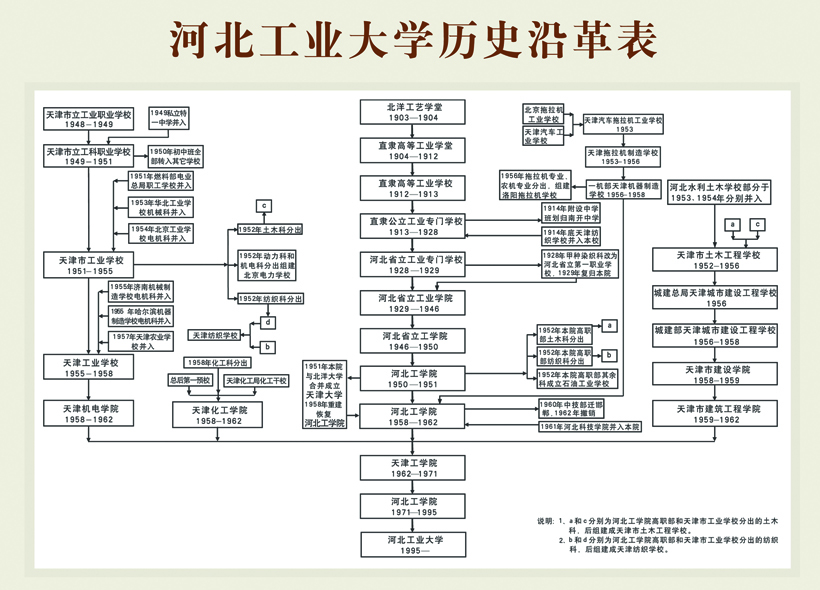
\includegraphics[width=0.5\textwidth]{figures/historyhebut}
    \caption{河北工业大学历史沿革}\label{fig:historyhebut}
\end{figure}

\section{标题3}
引用如这样\cite{song_score-based_2020}
\section{标题4}


\subsection{插表}
一般情况下,表格须通栏,即表格宽度与正文版面平齐,如下表所示。
\begin{table}
    \centering
    \caption{测试用例表}\label{tab:table_centered}
    \begin{tabularx}{\textwidth}{>{\centering\arraybackslash}X>{\centering\arraybackslash}X>{\centering\arraybackslash}X}
    \toprule
    列1 & 列2 & 列3 \\
    \midrule
    有效 & 001 & 通过 \\
    无效 & 002 & 未通过 \\
    \bottomrule
    \end{tabularx}
\end{table}
     %插入章节一
% !TeX root = ../HebutThesis_example.tex(此文件是被HebutThesis_example.tex调用的)
\chapter{插图插表及引用参考文献方法(仅供参考)}

\section{插图}
插图:一般情况下,在正文中,先见到图号和图的内容再展示图。
特殊情况须延后的插图不应跨节。

通常使用的函数图采用简化形式,称为简写函数图,例如图{\ref{fig:historyhebut}}以及图{\ref{fig:河北工业大学校门}}。
% 引用图的方法:在正文中插入\ref{tab:表的名称}
\begin{figure}[ht]
    \centering                                                      % 居中
    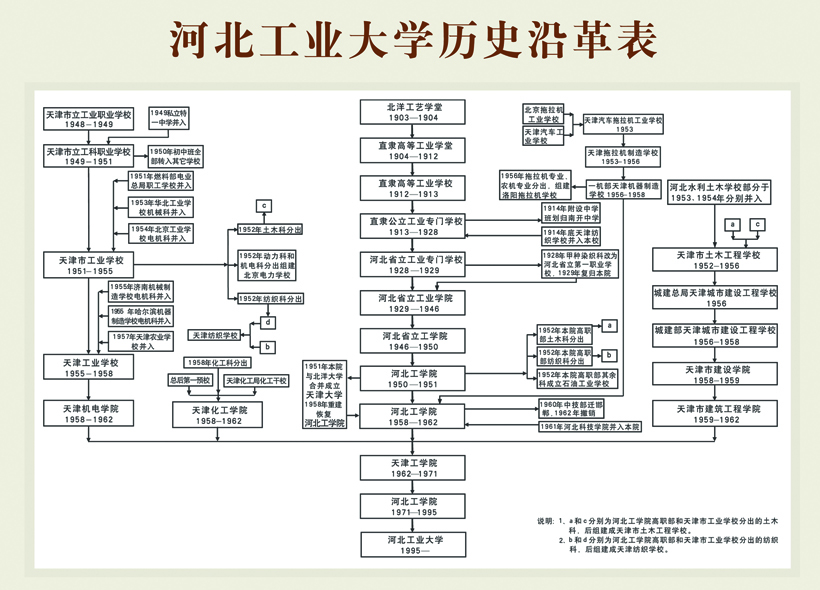
\includegraphics[width=0.5\textwidth]{figures/historyhebut}     % 页面宽度为文本宽度的0.5倍
    \caption{河北工业大学历史沿革}\label{fig:historyhebut}            % caption后为设定的图片名称,label后为图片文件名称
\end{figure}

\begin{figure}[ht]
    \centering
    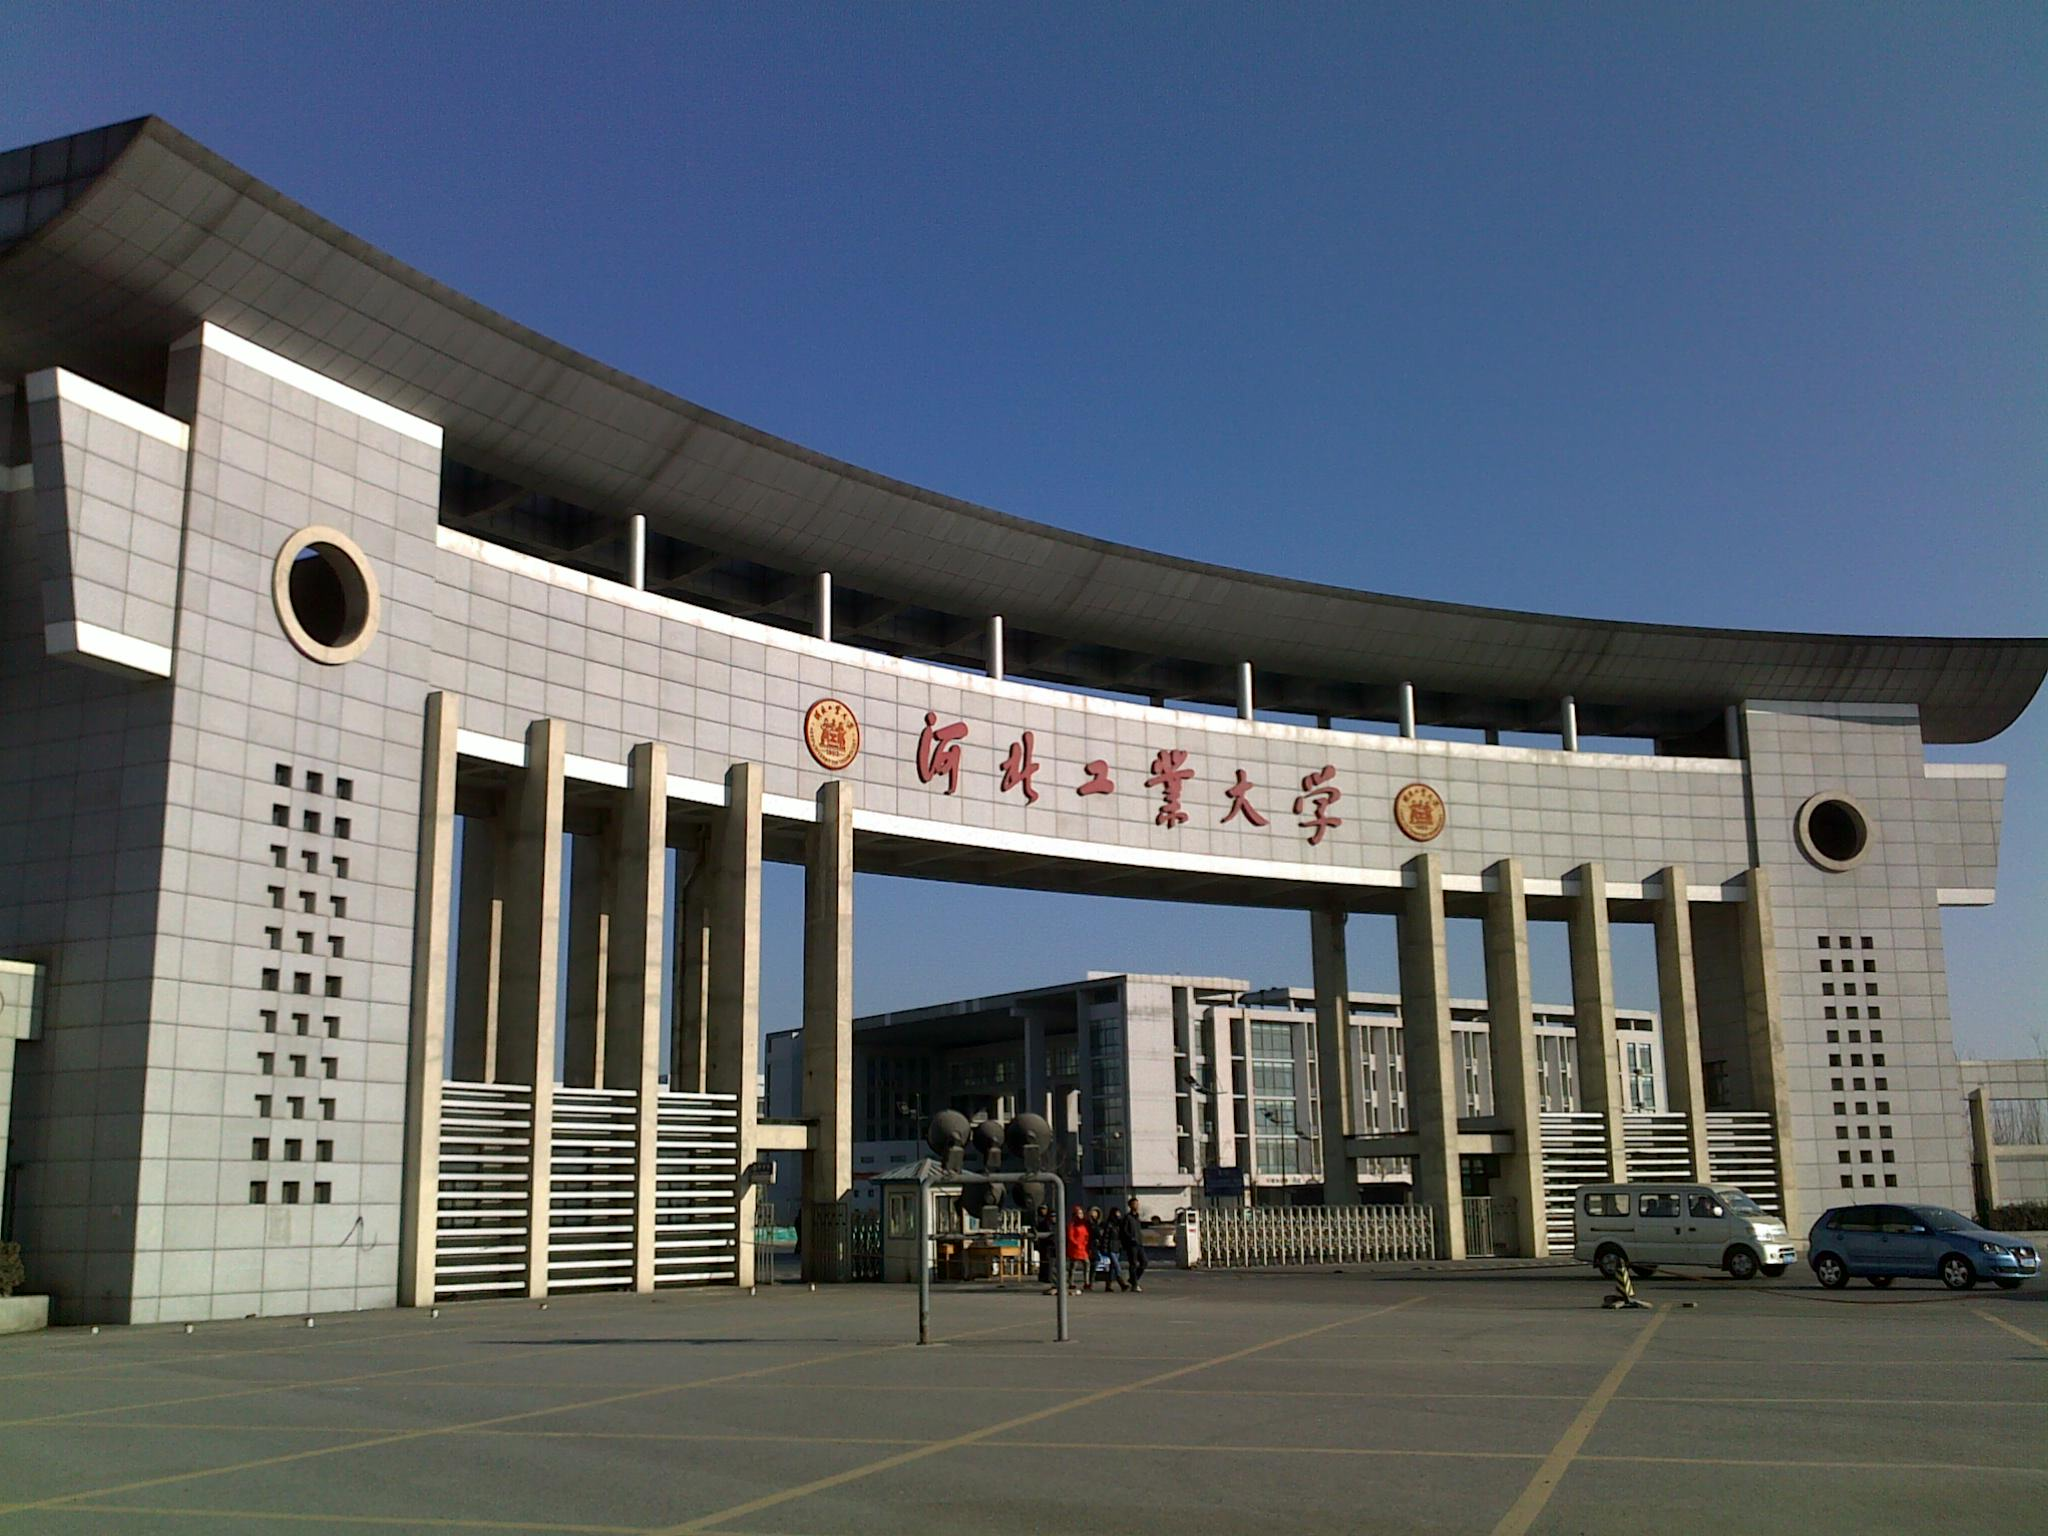
\includegraphics[width=\textwidth]{figures/河北工业大学校门}
    \caption{河北工业大学校门}\label{fig:河北工业大学校门}
\end{figure}

\section{插表}
一般情况下,表格须通栏,即表格宽度与正文版面平齐,
简单的表可以使用tabular包。如\ref{tab:table_example}所示,
复杂的可以使用tabularx包,如三线表\ref{tab:table_centered}所示。
% 引用表的方法:在正文中插入\ref{tab:表的名称}
两种包的区别:

使用tabular时,列宽基于内容或者指定的宽度,表格宽度自适应。

使用tabularx时,表格宽度固定,X格式列的宽度自动调整以适应表格总宽度。
允许指定表格的总宽度,X列会自动调整宽度,以填满指定的表格宽度。
适用于需要表格宽度匹配特定尺寸(如页面宽度)的场景。

\begin{table}[ht]
    \centering
    \caption{表格示例}
    \label{tab:table_example}
    \begin{tabular}{|l|c|r|}
    \hline
    左对齐 & 居中对齐 & 右对齐 \\ \hline
    数据1 & 数据2 & 数据3 \\
    数据4 & 数据5 & 数据6 \\ \hline
    \end{tabular}
\end{table}


\begin{table}
    \centering
    \caption{三线表示例}\label{tab:table_centered}      % caption后为设定的表格上名称,label后为表格标签
    \begin{tabularx}{\textwidth}{>{\centering\arraybackslash}X>{\centering\arraybackslash}X>{\centering\arraybackslash}X}
    % {\textwidth}用于调整表总宽度
    % >{\centering\arraybackslash}:这是列格式的预定义设置,
    % 用于使列中的内容居中。>{}用于在进入列前插入指定的命令,
    % 这里是\centering命令,用于使列中的文本居中对齐。\arraybackslash是必要的,
    % 因为\centering命令会重定义\\命令,而在表格中\\用于换行,
    % 所以需要\arraybackslash来恢复\\的原始功能,即结束当前行。
    \toprule
    列1 & 列2 & 列3 \\
    \midrule
    有效 & 001 & 通过 \\
    无效 & 002 & 未通过 \\
    文本1 & 文本2 & 长文本3的内容可能会更多,但这三列的宽度会自动平均分配。\\
    文本4 & 文本5 & 文本6 \\
    \bottomrule
    \end{tabularx}
\end{table}

\section{引用}
本文档中参考文献样式标准以GB/T 7714-2015为准,引用像这样\cite{song_score-based_2020}  % song_score-based_2020是biblography里的名字

文档中使用BibTeX来进行参考文献的引用,BibTeX是一种用于管理和格式化参考文献的工具,它使用特定的规则来结构化参考文献数据。
这些规则涉及到如何编写条目(每个参考文献的描述),条目类型(如书籍、文章等),以及字段(如作者、标题等)。
下面是一些基本使用方法:

BibTeX对不同类型的参考文献(期刊、图书、会议论文、未发表论文)等设定了不懂的类。
其中包括:@article表示期刊、@book表示有确定出版社的书籍、@booklet没有经过出版物出版的印刷作品、
@conference等同于@inproceedings表示会议文章等等。

可根据不同类型出版物的定义规范在../bibliography.bib文件中添加文献,并在这里引用即可自动在最后的参考文献部分生成reference list,像这样\cite{example2019}。




% !TeX root = ../HebutThesis_example.tex(此文件是被HebutThesis_example.tex调用的)
\chapter{chapter 3}
\section{section 1}
\subsection{subsection 1}
\subsection{subsection 2}
\section{section 2}
% !TeX root = ../HebutThesis_example.tex(此文件是被HebutThesis_example.tex调用的)
\chapter{chapter 4}
\section{section 1}
\subsection{subsection 1}
\subsection{subsection 2}
\section{section 2}

% 其他部分
\ctexset{
    chapter={
        name={},
        number = \arabic{chapter},
        format={\centering\bfseries\heiti\zihao{-3}},
        aftername={\quad}, 
        beforeskip={.5\baselineskip},
        afterskip={.5\baselineskip},
    }
}
\chapter*{结论}     % 不会自动添加到目录,且没序号
本文对...
             %插入结论
\addcontentsline{toc}{chapter}{结论}     %比如 \chapter{绪论} 的命令无法自动添加到目录,要手动将此条目添加到目录
% \bibliography{bibliography}
% \bibliographystyle{unsrt}
\printbibliography[title=参考文献,heading=bibintoc]           %插入参考文献
% !TeX root = ../HebutThesis_example.tex(此文件是被HebutThesis_example.tex调用的)
% 在此文件中编辑致谢中需要填写的内容
\chapter*{致谢}
% 以下替换为您论文致谢的内容
衷心感谢导师×××教授和xx系××教授对本人的精心指导。他们的言传身教将使我终生受益。

在河北工业大学……研究期间,承蒙xxx热心指导与帮助,不胜感激。

感谢×××××实验室主任×××教授,以及实验室全体老师和同学的热情帮助和支持!

本课题承蒙xxx基金资助,特此致谢。        %插入致谢
\addcontentsline{toc}{chapter}{致谢}     %手动添加到目录
\appendix                               %标记文档中附录部分的开始
% !TeX root = ../HebutThesis_example.tex(此文件是被HebutThesis_example.tex调用的)
% 在此文件中编辑您论文附录里需要填写的内容
\chapter{附录A标题}               %插入附录

\end{document}